\documentclass[12pt]{article}
 
\usepackage[margin=1in]{geometry}
\usepackage{amsmath,amsthm,amssymb}
\usepackage{unicode-math}
\usepackage{pgfplots}
 
\newcommand{\N}{\mathbb{N}}
\newcommand{\Z}{\mathbb{Z}}
 
\newenvironment{theorem}[2][Theorem]{\begin{trivlist}
\item[\hskip \labelsep {\bfseries #1}\hskip \labelsep {\bfseries #2.}]}{\end{trivlist}}
\newenvironment{lemma}[2][Lemma]{\begin{trivlist}
\item[\hskip \labelsep {\bfseries #1}\hskip \labelsep {\bfseries #2.}]}{\end{trivlist}}
\newenvironment{exercise}[2][Exercise]{\begin{trivlist}
\item[\hskip \labelsep {\bfseries #1}\hskip \labelsep {\bfseries #2.}]}{\end{trivlist}}
\newenvironment{problem}[2][Problem]{\begin{trivlist}
\item[\hskip \labelsep {\bfseries #1}\hskip \labelsep {\bfseries #2.}]}{\end{trivlist}}
\newenvironment{question}[2][Question]{\begin{trivlist}
\item[\hskip \labelsep {\bfseries #1}\hskip \labelsep {\bfseries #2.}]}{\end{trivlist}}
\newenvironment{corollary}[2][Corollary]{\begin{trivlist}
\item[\hskip \labelsep {\bfseries #1}\hskip \labelsep {\bfseries #2.}]}{\end{trivlist}}

\newenvironment{solution}{\begin{proof}[Solution]}{\end{proof}}
 
\begin{document}


\title{\LARGE Group Assignment 3} 
% replace X with the appropriate number
\author{\small Kirti Barman, Sourav Sharan, Vyoma Shah, Aditya Khadkikar \\ \small Group 15 - Introduction to Data Science} 
% if necessary, replace with your course title}

\maketitle

%%%%%%%%%%%%%%%%%%%%%%%%%%%%%%%%%%%%%%%%%%%%%%%%%%%%%

\begin{exercise}{1}
Consider a three state (1, 2, 3) Markov Chain with transition matrix
\[
P =
\begin{pmatrix}
0.5 & 0.5 & 0 \\
0.5 & 0 & 0.5 \\
0.5 & 0 & 0.5
\end{pmatrix}
\]
(a) Draw transition diagram. \\
(b) Find the stationary distribution $\pi$.\\
(c) Given that the chain is in state 1 at time 1, what is the probability
that the chain is in state 2 at time 4?\\
(d) Given that the chain is in state 1 at time 1, what is the expected
time until the chain is in state 3 the first time?\\
(e) What is the period of each state?\\
\end{exercise}
\begin{figure}
    \centering
    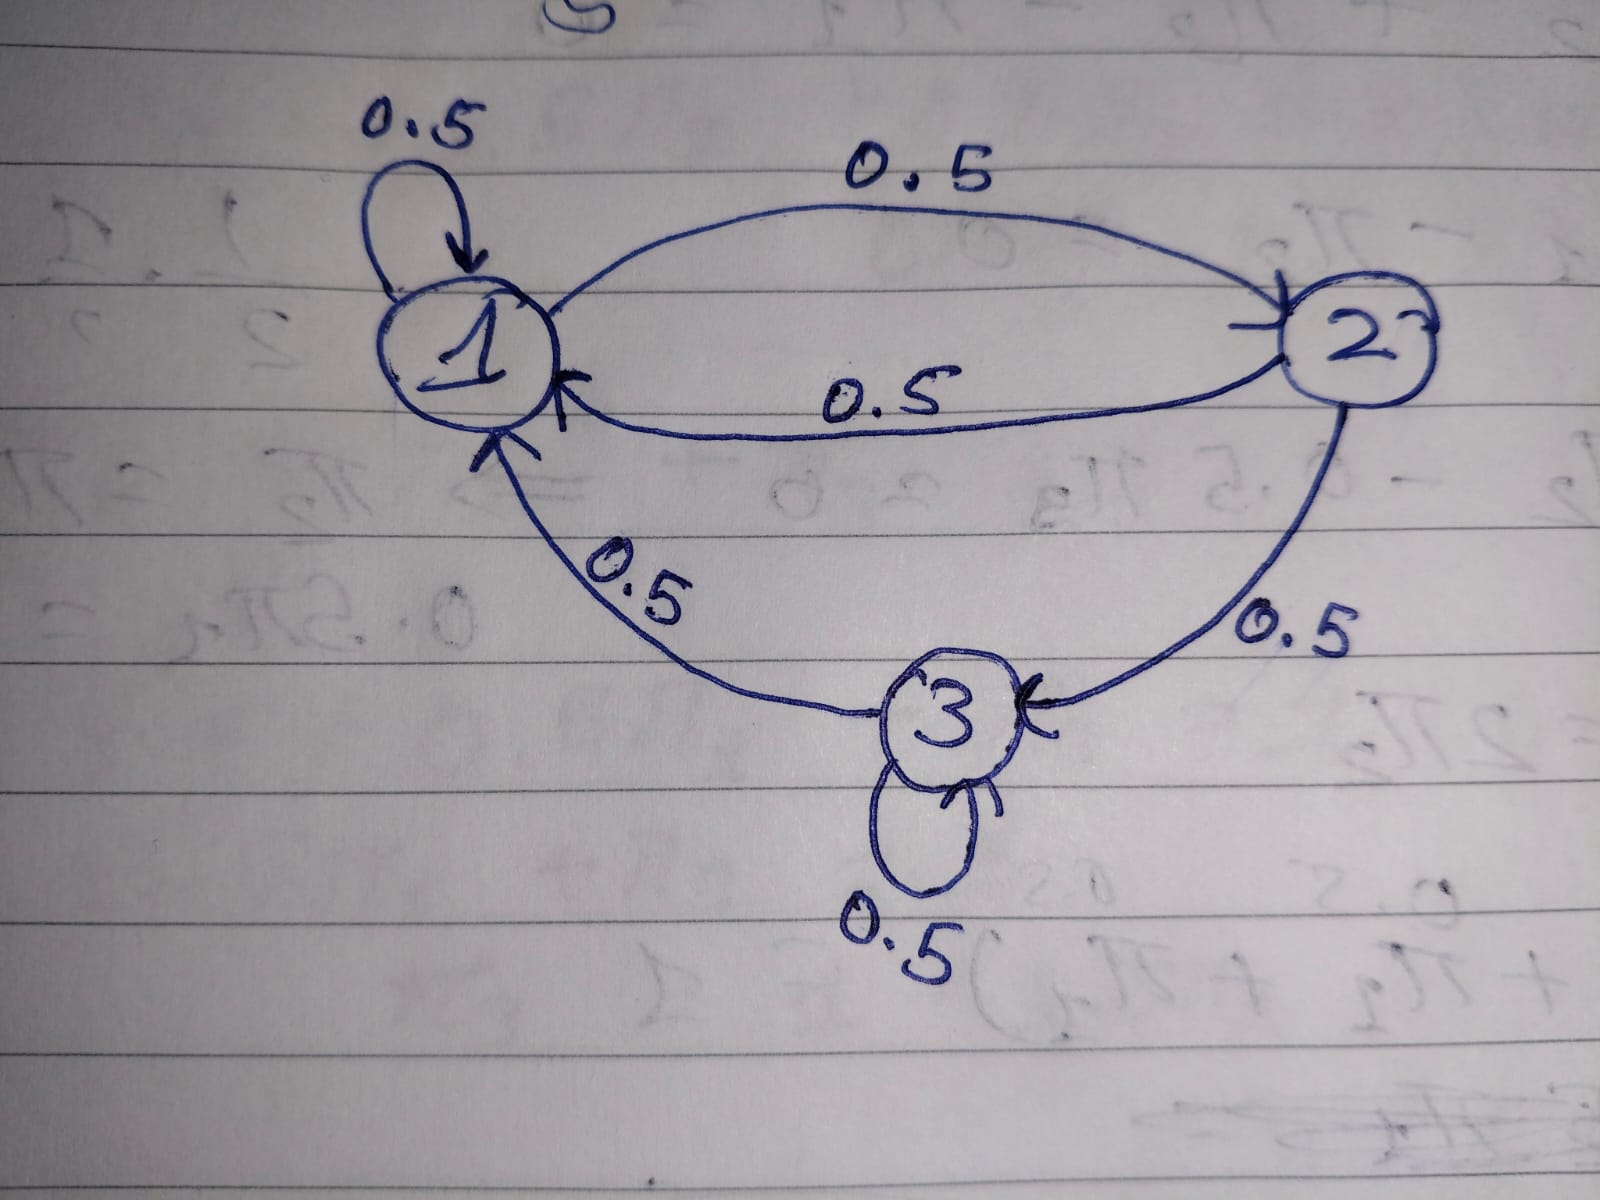
\includegraphics[width=0.4\linewidth]{Transition diagram.jpg}
    \caption{Transition Diagram}
    \label{fig:enter-label}
\end{figure}
\begin{solution}
Solving for Markov chain transition matrix P, 
\subsubsection*{(a) Transition Diagram:}
The transition diagram connects states based on the probabilities given in $P$:
\begin{itemize}
    \item State 1 transitions to itself (0.5) and to state 2 (0.5).
    \item State 2 transitions to state 1 (0.5) and state 3 (0.5).
    \item State 3 transitions to state 1 (0.5) and itself (0.5).
\end{itemize}


\subsubsection*{(b) Stationary Distribution:}
The stationary distribution $\pi = (\pi_1, \pi_2, \pi_3)$ satisfies\\ 
$$\pi P = \pi$$ 
Solving $\pi P = \pi$ for the matrix given above, we get the following set of equations:\\
$$\pi_1 = 0.5\pi_1 + 0.5\pi_2 + 0.5\pi_3$$\smallskip
$$\pi_2 = 0.5\pi_1$$\smallskip
$$\pi_3 = 0.5\pi_2 + 0.5\pi_3$$\smallskip
$$\pi_1 + \pi_2 + \pi_3 = 1 (Normalization).$$

Solving gives, \\ $$\pi = \left(\frac{1}{2}, \frac{1}{4}, \frac{1}{4}\right)$$

\subsubsection*{(c) State Transition Probability:}
Using 
\[
P^4 =
\begin{pmatrix}
0.5 & 0.25 & 0.25 \\
0.5 & 0.25 & 0.25 \\
0.5 & 0.25 & 0.25
\end{pmatrix}
\]
The probability of being in state 2 at time 4 starting from state 1 is 0.25.

\subsubsection*{(d) Expected Time to State 3:}
To find the expected time to reach state 3 given that we started at state 1, we set up a system of equations. This aims at finding the expected number of steps from a state i to the destination, i being the state space which we have. Those are the unknown variables in the system of equations. It is set up like below:

\[
m_{1\rightarrow3} = 1 + p_{1\rightarrow2}m_{2\rightarrow3} + p_{1\rightarrow1}m_{1\rightarrow3}
\]
\[
m_{2\rightarrow3} = 1 + p_{2\rightarrow1}m_{1\rightarrow3}
\]
\[
m_{3\rightarrow3} = 0
\]

From the above equations, $m_{3\rightarrow3}$ is 0, as we are already at our desired destination node. We substitute in the values for the probabilities, as we know them from the transition matrix.

\[
m_{1\rightarrow3} = 1 + 0.5m_{2\rightarrow3} + 0.5m_{1\rightarrow3}
\]
\[
m_{2\rightarrow3} = 1 + 0.5m_{1\rightarrow3}
\]

Moving the unknown terms to one side, we get:

\[
0.5m_{1\rightarrow3} - 0.5m_{2\rightarrow3} = 1
\]
\[
-0.5m_{1\rightarrow3} + m_{2\rightarrow3} = 1 
\]

Solving the equations, we get $m_{1\rightarrow3} = 6$, and $m_{2\rightarrow3} = 4$. \\

Therefore, the expected time to reach state 3 from state 1 is 6.

\subsubsection*{(e) Period of Each State:}
To calculate the period of each state, we can see the possible routes that can be taken to start from the given state, and return back. \\

For state 1, some of the possible routes are 1->1 (1 step), 1->2->1 (2 steps), 1->2->3->1 (3 steps). The greatest common divisor of these step counts is 1, so the period of the first state is 1.

For state 2, possible routes are 2->1->2 (2 steps), 2->3->1->2 (3 steps). The greatest common divisor of 2 and 3 is 1, so the period of state 2 is 1.

Lastly, for state 3, possible routes are 3->3 (1 step), 3->1->2->3 (3 steps). This is sufficient, as the greatest common divisor of 1 and 3 is 1, so the period of state 3 is also 1. \\

Hence, all states have a period of 1.
\end{solution}

\newpage

\begin{exercise}{2}
Assume that we are trying to classify a binary outcome $( Y )$, i.e., our data is of the form $( (X, Y) \sim F_{X,Y} )$, where $( Y \in {0, 1} )$ and $( X \in \mathbb{R}^d )$. We have used data to train a classifier $( g(X) )$. We can evaluate the performance of the classifier using i.i.d. testing data, $( (X_1, Y_1), \ldots, (X_n, Y_n) )$. We are interested in estimating the following quantities:\\\\
Precision: $( P(Y = 1 | g(X) = 1) )$\\
Recall: $( P(g(X) = 1 | Y = 1) )$\\\\
(a) Write down the empirical version of the precision and recall.\\
(b) Let us now think that the variable Y denotes if a battery’s health
has deteriorated or not, and let X denote a bunch of constructed
health indicators about the battery. If the model g(X) predicts
that the battery has deteriorated you need to run a test to confirm
this. The cost of running the test is \textit{c} when the battery is
not deteriorated. On the other hand, if the battery is in fact deteriorated
and the test is not run, the battery will die during use
and the cost of this is \textit{d}. \\
Define a random variable representing the cost of the decision g(X) and write down the formula for the
expected cost in terms of the precision and recall.\\
(c) Advanced question: can you produce a confidence interval for the
expected cost? What about the precision and the recall?
\end{exercise}

\begin{solution}
\subsubsection*{Precision and Recall:}
\[
\text{Precision} = \frac{N(Y=1 \cap g(X)=1, m)}{m},
\]
where m represents the total subset of points from the predictions by the model g(x) in which a 1 was predicted (TP + FP). The above equation is based on the Long Term Relative Frequency, aiming to estimate the probability equation of precision empirically.
\[
\text{Recall} = \frac{N(g(x)=1 \cap Y=1,n)}{n},
\]
where n represents the number of points from the testing dataset that match the label 1 (TP + FN). Similar to precision, this is the empirical formula, and can be used to estimate the probability equation for recall.
\subsubsection*{Cost Function:}
The cost of running the test is c when a battery is not deteriorated, however g(x) predicted the opposite. This refers to the model returning false positives (FP). Secondly, the cost d occurs when the battery is actually deteriorated, but predicted as functional (test not run), hence corresponding to the false negatives (FN). 

A cost function can be defined as having a combination of the empirical precision $\hat{P}$ and recall $\hat{R}$ depending on what the placeholders for c and d are. If one has a higher cost than the other, it can be weighted more heavily, for it being a more significant part of the cost function. This is with a parameter $0 \leq \alpha \leq 1$. The expectation of the random variable C representing the cost function, is in terms of of the tradeoff combination as (1-Precision) and (1-Recall) is so that the overall cost function can be made with respect to the false negatives and false positives. The precision and recall values both initially have the true positives in the numerator. 

\[
E[C] = \alpha (1 - \hat{P}) + (1 - \alpha)(1 - \hat{R}).
\]
\[
E[C] = \alpha \frac{TP+FP-TP}{TP + FP} + (1 - \alpha)\frac{TP+FN-TP}{TP + FN}.
\]
\[
= \alpha (\frac{N(g(X)=1 \cap Y=0,m)}{m}) + (1 - \alpha)(\frac{N(g(X)=0 \cap Y=1,n)}{n}),
\]

where 1 represents the label "deteriorated", and 0 represents that the battery is "not deteriorated".

\subsubsection*{Confidence Intervals:}
With $\hat{P}$ being the empirically estimated precision, confidence intervals are found using the binomial proportion interval:
\[
P \in \left[ \hat{P} - z_{1-\alpha/2} \cdot \sqrt{\frac{\hat{P}(1 - \hat{P})}{m}}, \hat{P} + z_{1-\alpha/2} \cdot \sqrt{\frac{\hat{P}(1 - \hat{P})}{m}} \right].
\]
where m is the same value as used in the empirical precision formula (the number of predictions that had label 1). \\

For recall, in a similar manner, the same confidence interval is described as the following:
\[
R \in \left[ \hat{R} - z_{1-\alpha/2} \cdot \sqrt{\frac{\hat{R}(1 - \hat{R})}{n}}, \hat{R} + z_{1-\alpha/2} \cdot \sqrt{\frac{\hat{R}(1 - \hat{R})}{n}} \right],
\]
where n is the number of points in the testing dataset that are labelled 1.
\end{solution}

\newpage

\begin{exercise}{3}
Show that two $d$-dimensional zero-mean, unit-variance Gaussian random vectors $X$ and $Y$ are nearly orthogonal by calculating their dot product $X^\top Y$ and bounding the probability that it exceeds $\epsilon$.
\end{exercise}

\begin{solution}
\textbf{Dot Product Distribution:} The dot product $X^\top Y \sim \mathcal{N}(0, d)$.

\subsubsection*{Bounding Probability:}
Using Gaussian tail bounds:
\[
P(|X^\top Y| > \epsilon) \leq 2 \exp\left(-\frac{\epsilon^2}{2d}\right).
\]
This shows that $X$ and $Y$ are nearly orthogonal for large $d$.
\end{solution}

\newpage

\begin{exercise}{4}
Prove that $u_i u_i^\top$ is rank 1, $U = \sum_{i=1}^r u_i u_i^\top$ is rank $r$, and perform SVD on $U$.
\end{exercise}

\begin{solution}
\textbf{Rank of $u_i u_i^\top$:}
The outer product $u_i u_i^\top$ spans a 1-dimensional subspace, so it has rank 1.

\textbf{Rank of $U = \sum_{i=1}^r u_i u_i^\top$:}
If $u_1, \dots, u_r$ are orthonormal, $U$ spans an $r$-dimensional subspace, giving $\text{rank}(U) = r$.

\textbf{SVD of $U$:}
The singular value decomposition of $U$ is $U = U \Sigma U^\top$, where $U$ contains the singular vectors.
\end{solution}

\newpage

\begin{exercise}{5}
For $X \sim \text{Uniform}(B_1)$ (unit ball) and $Y = \|X\|_2$, find the distribution function of $Y$, analyze $\ln(1/Y)$, and calculate $E[\ln(1/Y)]$.
\end{exercise}

\begin{solution}
\textbf{Distribution Function of $Y$:}
The cumulative distribution function of $Y$ is:
\[
F_Y(y) = y^d, \quad 0 \leq y \leq 1.
\]

\textbf{PDF of $\ln(1/Y)$:}
Using $y = e^{-z}$, the PDF is:
\[
f_Z(z) = d e^{-dz}.
\]

\textbf{Expected Value:}
The expected value is:
\[
E[\ln(1/Y)] = \frac{1}{d}.
\]
\end{solution}
\end{document}